% MATH 201 Lab notes (c) by Carlos Contreras And Philippe Gaudreau
% MATH 201 Lab notes is licensed under a 
% Creative Commons Attribution 4.0 International license.
% CC BY 4.0

% You should have received a copy of the license along with this
% work. If not, see <http://creativecommons.org/licenses/by/4.0/>.

\documentclass[11pt]{article}
% MATH 201 Lab notes (c) by Carlos Contreras And Philippe Gaudreau
% MATH 201 Lab notes is licensed under a 
% Creative Commons Attribution 4.0 International license.
% CC BY 4.0

% You should have received a copy of the license along with this
% work. If not, see <http://creativecommons.org/licenses/by/4.0/>.

%% libraries
\usepackage[utf8x]{inputenc}
\usepackage{xcolor}
\usepackage[left=1.5cm,right=1.5cm,top=2.0cm,bottom=1.5cm,headheight=110pt]{geometry}
\usepackage{amsmath}
\usepackage{amssymb}
\usepackage{graphicx}
\usepackage{xifthen}
\usepackage{sverb}
\usepackage{fancyhdr}
\usepackage{mdframed}
\usepackage{textcomp}

%%%%%%%%%%%%%%%%%%%%%%%%%%%%%%%%%%%%%%%%%%%%%%%%%%%%%%%%%%%%%%%%%%%%%%%
% PDF compiling
\usepackage{ifpdf}
\ifpdf %
        \DeclareGraphicsExtensions{.pdf}%
\else %
        \DeclareGraphicsExtensions{.eps,.ps}%
\fi

%%%%%%%%%%%%%%%%%%%%%%%%%%%%%%%%%%%%%%%%%%%%%%%%%%%%%%%%%%%%%%%%%%%%%%%
% Figures path
\graphicspath{{figures/}}

%%%%%%%%%%%%%%%%%%%%%%%%%%%%%%%%%%%%%%%%%%%%%%%%%%%%%%%%%%%%%%%%%%%%%%%
% Problem counter
\newcounter{Problem}
\setcounter{Problem}{0}

%%%%%%%%%%%%%%%%%%%%%%%%%%%%%%%%%%%%%%%%%%%%%%%%%%%%%%%%%%%%%%%%%%%%%%%
% Definitions
\def\LabSolutions{\clearpage \newpage \begin{center} {\Large \it Solutions} \end{center} \setcounter{Problem}{0}}
\def\QuizSolutions{\newpage \begin{center} {\Large \it Solutions} \end{center} \setcounter{Problem}{0}}
\def\degree{\textdegree}
\def\grade#1{\begin{flushright} {\small [#1]}\\ \end{flushright} \vspace{-10pt}}
\def\codecolor{red!50!black}
\def\code#1{\textcolor{\codecolor}{\tt #1}}
\def\examname#1{%
                \ifnum\value{page}>1%
                    \newpage%
                \else%
                    \vspace*{5pt}%
                \fi%
                \large \textbf{#1} \setcounter{Problem}{0}\vspace{10pt}}
\def\topic#1{\par\needspace{2\baselineskip} \noindent \textsl{\footnotesize #1}}

 
%%%%%%%%%%%%%%%%%%%%%%%%%%%%%%%%%%%%%%%%%%%%%%%%%%%%%%%%%%%%%%%%%%%%%%%
% Environments
\newenvironment{problem}%
     {\stepcounter{Problem}%
      \begin{list}{\textbf{\arabic{Problem}}.~}{}%
      \item}%
     {\end{list}\vspace*{5pt}}

\newenvironment{solution}%
     {\indent \textit{Solution} \newline}%
     {\begin{flushright}$\blacksquare$\end{flushright}}

\newenvironment{preamble}%
     {\vspace*{1em}\begin{mdframed}[leftmargin=1cm,rightmargin=1cm]}%
     {\end{mdframed}\vspace*{1em}}

\newenvironment{multchoice}%
     {\begin{enumerate} \addtolength{\leftskip}{2em} \renewcommand{\labelenumi}{(\alph{enumi})}}
     {\end{enumerate}}

\newenvironment{formulaitem}%
     {\setlength{\leftmargini}{1.5em}\begin{itemize}%
      \setlength\itemindent{-\itemindent}%
      \renewcommand{\labelitemi}{$\rightarrow$}}%
     {\end{itemize}}


%%%%%%%%%%%%%%%%%%%%%%%%%%%%%%%%%%%%%%%%%%%%%%%%%%%%%%%%%%%%%%%%%%%%%%%
% New theorems
\newtheorem{theorem}{Theorem}


\makeatletter

%%%%%%%%%%%%%%%%%%%%%%%%%%%%%%%%%%%%%%%%%%%%%%%%%%%%%%%%%%%%%%%%%%%%%%%
%% New commands
\newcommand*{\course}[1]{\gdef\@course{#1}}
\newcommand*{\coursecode}[1]{\gdef\@coursecode{#1}}
\newcommand*{\term}[1]{\gdef\@term{#1}}
\newcommand*{\instructor}[1]{\gdef\@instructor{#1}}
\newcommand*{\lqnumber}[1]{\gdef\@lqnumber{#1}}
\newcommand*{\labtitle}[1]{\gdef\@labtitle{#1}}
\newcommand*{\quizversion}[1]{\gdef\@quizversion{#1}}
\newcommand*{\probleminfo}[1]{\noindent \textsl{\footnotesize #1}}

% Title header for labs
\newcommand\makelabtitle{%
  \begin{flushleft}%
  {\scshape \@coursecode~\@course~-- University of Alberta}\\%
  {\scshape \@term~-- Labs -- \@instructor}\\%
  {\scshape Authors: Carlos Contreras and Philippe Gaudreau}%
  \end{flushleft}%
  \begin{center}%
  {\Large \bf \@lqnumber:~\@labtitle}%
  \end{center}%
  \thispagestyle{empty}%
  \global\let\@course\@empty%
  \global\let\@labtitle\@empty%
}

% Title header for quizzes
\newcommand\makequiztitle{%
  \begin{flushleft}%
  {\scshape \@coursecode~\@course~-- University of Alberta}\\%
  {\scshape \@term~-- Labs -- \@instructor}\\%
  \end{flushleft}%
  \begin{center}%
  {\Large \bf \@lqnumber} \marginpar{\tiny\tt [\@quizversion]}%
  \end{center}%
  \thispagestyle{empty}%
  \global\let\@course\@empty%
  \global\let\@quizversion\@empty%
}

%%%%%%%%%%%%%%%%%%%%%%%%%%%%%%%%%%%%%%%%%%%%%%%%%%%%%%%%%%%%%%%%%%%%%%%
% Fancy header package
\fancyhead[L]{\small {\scshape \@coursecode~-- \@lqnumber~-- \@term~-- \@instructor}}
\pagestyle{fancy}

\makeatother


\usepackage{hyperref}
\usepackage{cancel}


\begin{document}

\course{Differential Equations}
\coursecode{MATH 201}
\term{Winter 2018}
\instructor{Carlos Contreras}
\lqnumber{Lab 8}
\labtitle{LT: discontinuous functions and Dirac delta function}
\makelabtitle



\topic{Discontinuous functions}

\begin{problem}
Express the given function using window and step functions and compute its Laplace transform
\begin{equation*}
g(t) = \begin{cases}
0, & 0<t<1, \\
2, & 1<t<2, \\
1, & 2<t<3, \\
3, & 3<t.
\end{cases}
\end{equation*}
\end{problem}




\begin{problem}
Determine the current as a function of time t for the given RLC series circuit. Plot the solution. The current $I(t)$ in a RLC series circuit is governed by the initial value problem
\begin{equation*}
I^{\prime \prime}(t)+2I^{\prime}(t) +2I(t)=g(t); \quad I(0)=10, \quad I^{\prime}(0) = 0,
\end{equation*}
where,
\begin{equation*}
g(t) = \begin{cases} 
20, &\quad 0<t<3\pi \\
0, &\quad 3\pi<t<4\pi \\
20, &\quad 4\pi<t
\end{cases}.
\end{equation*}
\end{problem}






\begin{problem}
Solve the initial value problem
\begin{equation*}
y^{\prime \prime}(t)+4y(t)=f(t); \quad y(0)=0, \quad y^{\prime}(0) = 0,
\end{equation*}
where,
\begin{equation*}
f(t) = \begin{cases} 
2t, &\quad 0\leq t<2 \\
4, &\quad 2 \leq t 
\end{cases}.
\end{equation*}
\end{problem}

\topic{Dirac delta function}

\begin{problem}
Evaluate the following integral
\begin{equation*}
\int_{-\infty}^{\infty} \sin(3t)\delta(t-\pi/2) d t.
\end{equation*}
\end{problem}





\begin{problem}
Solve the given symbolic initial value problem
\begin{equation*}
y^{\prime \prime} + 2 y^{\prime} - 3 y = \delta(t-1) - \delta(t-2) , \quad y(0) =2 , \quad y^{\prime}(0) = -2.
\end{equation*}
\end{problem}


\begin{problem}
Solve the given symbolic initial value problem
\begin{equation*}
y^{\prime \prime} + 5 y^{\prime} - 6 y = e^{-t}\delta(t-2), \quad y(0) =2 , \quad y^{\prime}(0) = -5.
\end{equation*}
\end{problem}






%%%%%%%%%%%%%%%%%%%%%%%%%%%%%%%%%%%%%%%%%%%%%%%%%%%%%%%%%%%%%%%%%%%%%%%%%%%%%%%%%%%%%%%%%%%%%%%%%%%



\LabSolutions


Theory and problems from: Nagel, Saff \& Sneider, \textit{Fundamentals of Differential Equations}, Eighth Edition, Adisson--Wesley.


\begin{preamble}
\begin{formulaitem}

\item The \textbf{unit step function} $u(t)$ is defined by
\begin{equation*}
u(t)=\left\{\begin{array}{ll}
             0, & t<0, \\
             1, & 0<t.
            \end{array} \right. 
\end{equation*}


\item The \textbf{rectangular window function} (or square pulse) $\Pi_{a,b}(t)$ is defined by
\begin{equation*}
\Pi_{a,b}(t)= u(t-a) - u(t-b) = \left\{\begin{array}{ll}
             0, & t<a, \\
             1, & a<t<b, \\
             0, & b<t.
            \end{array} \right. 
\end{equation*}

\item The \textbf{Dirac delta function} $\delta(t)$ is characterized by
\begin{equation*}
\delta(t) = \begin{cases}
0 , & t \neq 0 \\
\infty, & t = 0 
\end{cases},
\end{equation*}
and
\begin{equation*}
\int_{-\infty}^{\infty} f(t) \delta(t-a) d t = f(a).
\end{equation*}

\item The Dirac delta function is the \textbf{derivative} of the unit step function 
\begin{equation*}
\dfrac{ d}{ d t} u(t-a) = \delta(t-a).
\end{equation*}

\item Brief \textbf{table of Laplace Transforms}.

% \begin{table}[ht]
\renewcommand{\arraystretch}{1.5}
\setlength{\tabcolsep}{10pt}
\begin{center}
\begin{tabular}{|ll|ll|}
\hline
$f(t)$ & $F(s)=\mathcal{L}\{f\}(s)$ & $f(t)$ & $F(s)=\mathcal{L}\{f\}(s)$ \\
\hline
$e^{at}f(t)$ & $F(s-a)$                                   &  $1$ & $\frac{1}{s}$ \\
$f'(t)$ & $sF(s)-f(0)$                                    &  $e^{at}$ & $\frac{1}{s-a} \qquad s>a$\\ 
$f''(t)$ & $s^{2}F(s)-sf(0)-f'(0)$                        &  $t^{n}$ & $\frac{n!}{s^{n+1}}$ \\
$t^{n}f(t)$ & $(-1)^{n}F^{(n)}(s)$                        &  $\sin bt$ & $\frac{b}{s^{2}+b^{2}}$ \\
$(f*g)(t)$ & $F(s)G(s)$                                   &  $\cos bt$ & $\frac{s}{s^{2}+b^{2}}$ \\
$u(t-a)$ & $\frac{e^{-as}}{s}$                            &  $e^{at}t^{n}$ & $\frac{n!}{(s-a)^{n+1}} \qquad s>a$ \\
$f(t-a)u(t-a)$ & $e^{-as}F(s)$                            &  $e^{at}\sin bt$ & $\frac{b}{(s-a)^{2}+b^{2}} \qquad s>a$ \\
$\delta(t-a)$ & $e^{-as}$                                 &  $e^{at}\cos bt$ & $\frac{s-a}{(s-a)^{2}+b^{2}} \qquad s>a$ \\
$\int_{0}^{s}f(\tau)d\tau$ & $\frac{1}{s}F(s)$            &  $\sinh bt$ & $\frac{b}{s^{2}-b^{2}}$ \\
$\frac{1}{t}f(t)$ & $\int_{s}^{\infty}F(\sigma)d\sigma$   &  $\cosh bt$ & $\frac{s}{s^{2}-b^{2}}$ \\
\hline 
\end{tabular}
\end{center}
% \caption{Brief table of Laplace Transforms.}
% \end{table}

\end{formulaitem}
\end{preamble}

\newpage

\begin{problem}
Express the given function using window and step functions and compute its Laplace transform
\begin{equation*}
g(t) = \begin{cases}
0, & 0<t<1, \\
2, & 1<t<2, \\
1, & 2<t<3, \\
3, & 3<t.
\end{cases}
\end{equation*}
\end{problem}
\begin{solution}
Expressing $g(t)$ in unit step functions
\begin{eqnarray*}
g(t) & = & (0) \Pi_{0,1}(t) + (2)\Pi_{1,2}(t) + (1)\Pi_{2,3}(t) + (3) u(t-3) \\
& = & 2(u(t-1)-u(t-2)) + (u(t-2)-u(t-3)) + 3 u(t-3) \\
& = & 2u(t-1)-u(t-2)+2 u(t-3).
\end{eqnarray*}
Hence
\begin{eqnarray*}
{\cal L}\{ g(t) \} & = & 2{\cal L}\{ u(t-1) \}-{\cal L}\{ u(t-2) \} +2{\cal L}\{ u(t-3) \} \\
     & = & \boxed{\dfrac{2e^{-s}}{s}-\dfrac{e^{-2s}}{s} +\dfrac{2e^{-3s}}{s}}
\end{eqnarray*}
\end{solution}





\begin{problem}
Determine the current as a function of time t for the given RLC series circuit. Plot the solution. The current $I(t)$ in a RLC series circuit is governed by the initial value problem
\begin{equation*}
I^{\prime \prime}(t)+2I^{\prime}(t) +2I(t)=g(t); \quad I(0)=10, \quad I^{\prime}(0) = 0,
\end{equation*}
where,
\begin{equation*}
g(t) = \begin{cases} 
20, &\quad t<3\pi \\
0, &\quad 3\pi<t<4\pi \\
20, &\quad 4\pi<t
\end{cases}.
\end{equation*}
\end{problem}
\begin{solution}
We can rewrite the function $g(t)$ using unit step function as follows:

\begin{equation*}
g(t) = 20-20 u(t-3\pi) +20 u(t-4\pi) = 20(1-u(t-3\pi) + u(t-4\pi))
\end{equation*}

Hence our IVP can be rewritten as:

\begin{equation*}
I^{\prime \prime}(t)+2I^{\prime}(t) +2I(t)=20(1-u(t-3\pi) + u(t-4\pi)); \quad I(0)=10, \quad I^{\prime}(0) = 0,
\end{equation*}

Taking the Laplace transform on both sides of this equation, we obtain:
\begin{equation*}
{\cal L}^{}\{ I^{\prime \prime}(t) \} + 2{\cal L}^{}\{ I^{\prime }(t) \}+2 {\cal L}^{}\{ I(t) \} =20 ( {\cal L}^{}\{ 1 \}- {\cal L}^{}\{ u(t-3\pi) \} + {\cal L}^{}\{ u(t-4\pi) \})
\end{equation*}
Expanding, we obtain:

\begin{eqnarray*}
(s^2J(s)-sI(0)-I^{\prime}(0)) + 2 ( sJ(s)-I(0))+2 J(s) & = & 20 \left( \dfrac{1}{s}- \dfrac{e^{-3\pi s}}{s} + \dfrac{e^{-4\pi s}}{s}\right) \\
s^2J(s)-10s + 2sJ(s)-20+2 J(s) & = & \dfrac{20}{s}- \dfrac{20e^{-3\pi s}}{s} + \dfrac{20e^{-4\pi s}}{s} \\
\end{eqnarray*}
Isolating for $J(s)$, we obtain:
\begin{eqnarray*}
J(s)  =   \dfrac{20}{s(s^2+2s+2)}- \dfrac{20e^{-3\pi s}}{s(s^2+2s+2)} + \dfrac{20e^{-4\pi s}}{s(s^2+2s+2)} + \dfrac{10s+20}{s^2+2s+2}\\
\end{eqnarray*}
We need to find the partial fraction decomposition of  $F(s)=\dfrac{20}{s(s^2+2s+2)}$.

\begin{eqnarray*}
F(s)=\dfrac{20}{s(s^2+2s+2)} & = & \dfrac{As+B}{s^2+2s+2} + \dfrac{C}{s} \\
 & = & \dfrac{(As+B)s+ C(s^2+2s+2)}{s(s^2+2s+2)} \\
 & = & \dfrac{s^2(A+C) + s(B+2C) + 2C }{s(s^2+2s+2)}
\end{eqnarray*}
This leads to the following system of equations:

\begin{eqnarray*}
A+C &= &0\\
B+2C & = & 0\\
2C & = & 20
\end{eqnarray*}
This can easily be solve. $A=-10$,$B=-20$ and $C=10$
Hence:

\begin{eqnarray*}
J(s)  & = &   -\dfrac{10s+20}{s^2+2s+2} + \dfrac{10}{s} -F(s)e^{-3\pi s} +F(s)e^{-4\pi s} + \dfrac{10s+20}{s^2+2s+2} \\
& = &    \dfrac{10}{s} -F(s)e^{-3\pi s} +F(s)e^{-4\pi s} \\
\end{eqnarray*}

The inverse Laplace transform of $F(s)$ is given by:

\begin{eqnarray*}
f(t) = {\cal L}^{-1}\{ F(s) \} & = & {\cal L}^{-1}\left\{ -\dfrac{10s+20}{s^2+2s+2} + \dfrac{10}{s} \right\} \\
& = & {\cal L}^{-1}\left\{ \dfrac{-10(s+1)-10}{(s+1)^2+1}\right\} +10 {\cal L}^{-1}\left\{ \dfrac{1}{s}\right\}\\
& = & -10{\cal L}^{-1}\left\{ \dfrac{s+1}{(s+1)^2+1}\right\} -10 {\cal L}^{-1}\left\{ \dfrac{1}{(s+1)^2+1}\right\} +10 {\cal L}^{-1}\left\{ \dfrac{1}{s}\right\}\\
&=& -10e^{-t}\cos(t)-10e^{-t}\sin(t) +10
\end{eqnarray*}
We can now find the function $I(t)$ via the property $ {\cal L}^{-1}\{ e^{-as}F(s) \}(t) = f(t-a)u(t-a)$. Taking the inverse Laplace transform of our function $J(s)$, we obtain:

\begin{eqnarray*}
I(t) & = & {\cal L}^{-1}\{ J(s) \}  \\
& = & 10 {\cal L}^{-1}\left\{ \dfrac{1}{s}\right\}  -{\cal L}^{-1}\left\{ e^{-3\pi s} F(s)\right\} + {\cal L}^{-1}\left\{ e^{-4\pi s} F(s)\right\} \\
& = & 10 - \left(-10e^{-(t-3\pi)}\cancelto{\scriptstyle -\cos t}{\cos(t-3\pi)}-10e^{-(t-3\pi)}\cancelto{\scriptstyle -\sin t}{\sin(t-3\pi)} +10\right)u(t-3\pi) \\
& & + \left(-10e^{-(t-4\pi)}\cancelto{\scriptstyle \cos t}{\cos(t-4\pi)}-10e^{-(t-4\pi)}\cancelto{\scriptstyle \sin t}{\sin(t-4\pi)} +10\right)u(t-4\pi) \\
& = & 10 - \left(10e^{-(t-3\pi)}\cos(t)+10e^{-(t-3\pi)}\sin(t) +10\right)u(t-3\pi) \\
& & + \left(-10e^{-(t-4\pi)}\cos(t)-10e^{-(t-4\pi)}\sin(t) +10\right)u(t-4\pi) 
\end{eqnarray*} 
Hence,
\begin{gather*}
\boxed{I(t) = 10 - 10 u(t-3\pi) \left[ 1+e^{-(t-3\pi )} \left(\cos t+\sin t\right)\right] + 10 u(t-4\pi) \left[1-e^{-(t-4\pi)}(\cos t+\sin t)\right]}.
\end{gather*}

If we plot the function $I(t)$, we obtain:
\begin{figure}[h]
\begin{center}
\begin{tabular}{cc} 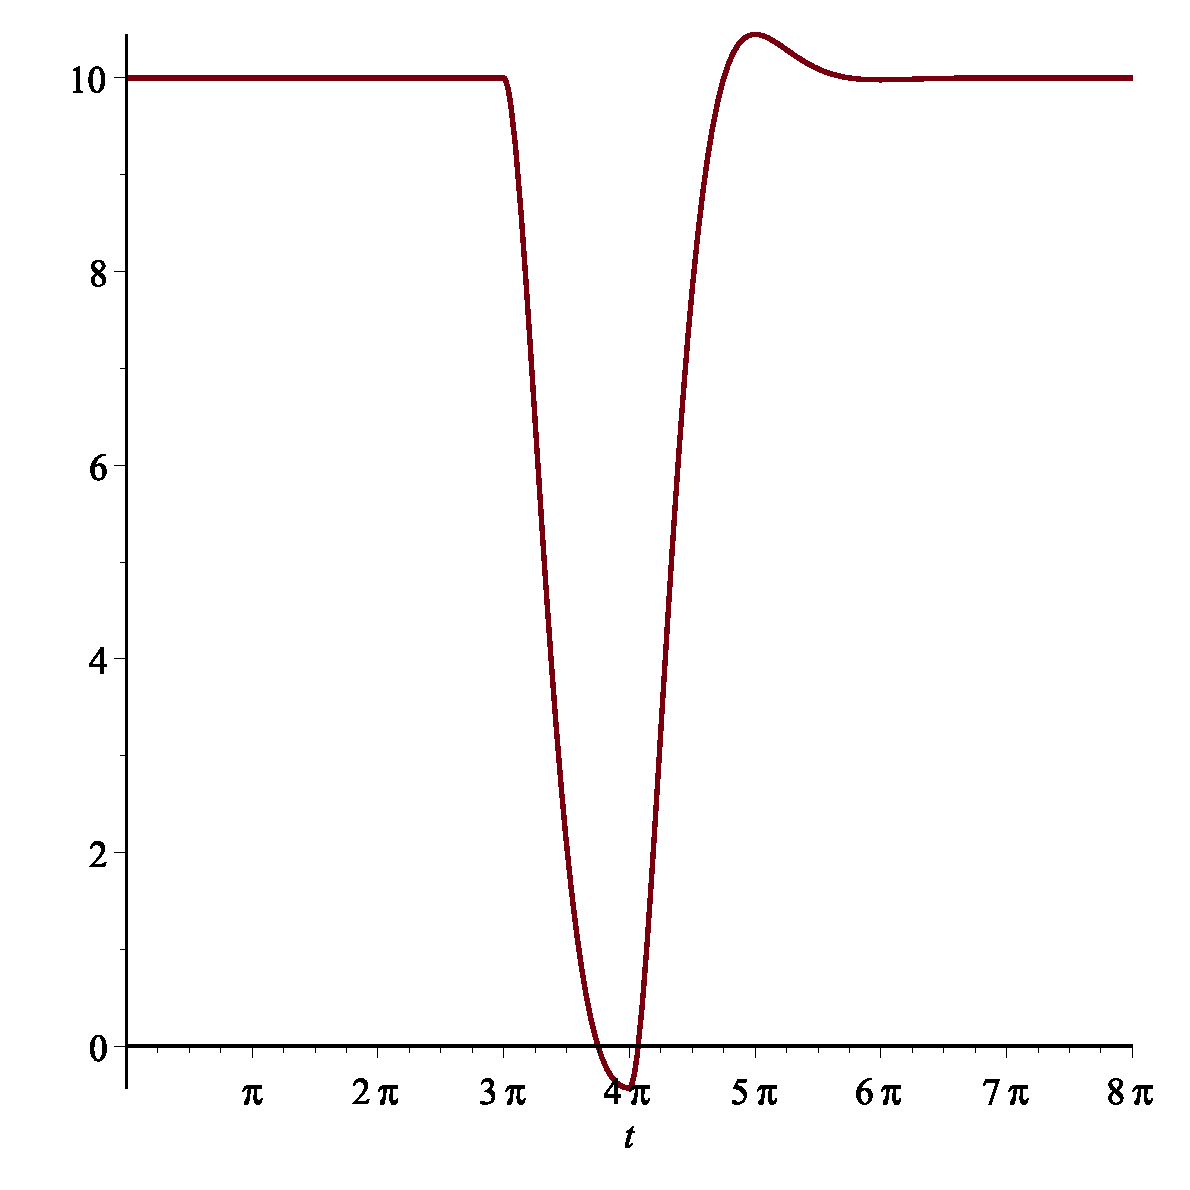
\includegraphics[width=0.5\textwidth]{lab09unitpulse} \\
\end{tabular}
\end{center}
\end{figure}
\end{solution}



\begin{problem}
Solve the initial value problem
\begin{equation*}
y^{\prime \prime}(t)+4y(t)=f(t); \quad y(0)=0, \quad y^{\prime}(0) = 0,
\end{equation*}
where,
\begin{equation*}
f(t) = \begin{cases} 
2t, &\quad 0\leq t<2 \\
4, &\quad 2 \leq t 
\end{cases}.
\end{equation*}
\end{problem}

\begin{solution}
The first step is to write $f(t)$ in terms of unit step functions
\[f(t)=2t+ (4 - 2t)u(t-2).\]
Note that $h(t)=4 -2t$ is not of the form $f(t-2)$ so using the property for $f(t-a)u(t-a)$ is not straight forward. A trick that will always work is to evalute $h(t+2)$\footnote{For the property $\mathcal{L}\{f(t-a)u(t-a)\}=F(s)e^{-as}$, we need the Laplace of $f(t)$, not the Laplce of $f(t-a)$. If we have $h(t)u(t-2)$, let $f(t-a)=h(t)$, then $f(t)=h(t+a)$. So $\mathcal{L}\{h(t)u(t-a)\}=\mathcal{L}\{f(t-a)u(t-a)\}=\mathcal{L}\{f(t)\}e^{-as}=\mathcal{L}\{h(t+a)\}e^{-as}$.},
\[h(t+2)=4-2(t+2)=-2t,\quad  \Rightarrow \quad \mathcal{L}\{h(t+2)\}=-\frac{2}{s^2},\]
and multiply by $e^{-2s}$
\[\mathcal{L}\{(4-2t)u(t-2)\} = -\frac{2}{s^2}e^{-2s}.\]
Then,
\[F(s)= \mathcal{L}\{2t\} + \mathcal{L}\{(4-2t)u(t-2)\}= \frac{2}{s^2} - \frac{2}{s^{2}}e^{-2s}=2\left( \frac{1}{s^2} - \frac{e^{-2s}}{s^{2}} \right)\]

Alternatively, we can write 
\[f(t)=2t(u(t)-u(t-2))+4u(t-2),\]
then, its Laplace transform (using the property for $tf(t)$) is, as expected,
\[F(s)=2(-1)\frac{d}{ds}\left[ \frac{1}{s} - \frac{e^{-2s}}{s} \right] + 4 \frac{e^{-2s}}{s} = 2 \left( \frac{1}{s^{2}} - \frac{e^{-2s}}{s^{2}} \right).\]


Next step is to apply Laplace of both side of the ODE
\[s^{2}Y(s) -0s-0+ 4 Y(s)=2 \left( \frac{1}{s^{2}} - \frac{e^{-2s}}{s^{2}} \right).\]
Isolating $Y(s)$ we have
\[Y(s)=\frac{2}{s^{2}(s^{2}+4)}- \frac{2}{s^{2}(s^{2}+4)} e^{-2s}=G(s) -G(s)e^{-2s}.\]
Is practical to take $e^{-as}$ terms as a common factor, since this only shift the inverse Laplace of $G(s)$.

Now we take the inverse Laplace transform of $G(s)$ using partial fractions
\[G(s)=\frac{2}{s^{2}(s^{2}+4)}=\frac{As+B}{s^{2}}+\frac{Cs+D}{s^{2}+4}= \frac{1}{2s^{2}}-\frac{1}{2(s^{2}+4)}.\]

Hence,
\[g(t)=\frac{1}{2}t-\frac{1}{4}\sin 2t\]

Finally,
\[y(t)=g(t)-g(t-2)u(t-2)\]
\[\Rightarrow \boxed{y(t)=\frac{t}{2}-\frac{\sin 2t}{4}- \left(\frac{t-2}{2}-\frac{\sin 2(t-2)}{4}\right)u(t-2)}.\]
\end{solution}



\begin{problem}
Evaluate the following integral
\begin{equation*}
\int_{-\infty}^{\infty} \sin(3t)\delta(t-\pi/2) d t.
\end{equation*}
\end{problem}
\begin{solution} 
Use the property of the Dirac delta function $\int_{-\infty}^{\infty} f(t) \delta(t-a) d t = f(a)$
\begin{equation*}
\int_{-\infty}^{\infty} \sin(3t)\delta(t-\pi/2) d t = \sin\left(\dfrac{3 \pi}{2} \right) =-1.
\end{equation*}
\end{solution}




\begin{problem}
Solve the given symbolic initial value problem
\begin{equation*}
y^{\prime \prime} + 2 y^{\prime} - 3 y = \delta(t-1) - \delta(t-2) , \quad y(0) =2 , \quad y^{\prime}(0) = -2.
\end{equation*}
\end{problem}
\begin{solution}
Applying a Laplace transform on both sides, we obtain:

\begin{equation*}
s^2 Y(s) -sy(0) - y^{\prime}(0) + 2sY(s) - 2y(0) - 3 Y(s) = e^{-s} - e^{-2s}
\end{equation*}
Subbing in our initial conditions, we obtain:

\begin{equation*}
s^2 Y(s) -2s +2 + 2sY(s) - 4 - 3 Y(s) = e^{-s} - e^{-2s}
\end{equation*}
Isolating $Y(s)$, we obtain:

\begin{eqnarray*}
Y(s) & = & \dfrac{2s+2}{s^2+2s-3}+ \dfrac{e^{-s}}{s^2+2s-3} - \dfrac{e^{-2s}}{s^2+2s-3}  \\
& = & \dfrac{2s+2}{(s+3)(s-1)}+\dfrac{1}{(s+3)(s-1)}e^{-s} - \dfrac{1}{(s+3)(s-1)}e^{-2s}  \\
\end{eqnarray*}
Decomposing these functions into partial fractions,we obtain:
\begin{eqnarray*}
Y(s) & = & \left( \dfrac{1}{s-1} + \dfrac{1}{s+3} \right)+ \dfrac{1}{4}\left( \dfrac{1}{s-1} - \dfrac{1}{s+3} \right) e^{-s}  -\dfrac{1}{4} \left( \dfrac{1}{s-1} - \dfrac{1}{s+3} \right) e^{-2s} \\
\end{eqnarray*}
Taking the inverse Laplace transform using the property $${\cal L}^{-1} \left\{ G(s)e^{-as} \right\}(t) = g(t-a)u(t-a),$$ we have
\begin{equation*}
\boxed{y(t) = e^{t}+e^{-3t}   + \tfrac{1}{4} \left( e^{t-1}-e^{-3(t-1)} \right)u(t-1) - \tfrac{1}{4} \left( e^{t-2}-e^{-3(t-2)} \right)u(t-2)}.
\end{equation*}
\end{solution}





\begin{problem}
Solve the given symbolic initial value problem
\begin{equation*}
y^{\prime \prime} + 5 y^{\prime} - 6 y = e^{-t}\delta(t-2), \quad y(0) =2 , \quad y^{\prime}(0) = -5.
\end{equation*}
\end{problem}
\begin{solution}
Recall the property $\mathcal{L}\{e^{at}f(t)\}=F(t-a)$. Then, applying a Laplace transform on both sides, we obtain
\begin{equation*}
Y(s)=\frac{2s+5}{s^{2}+5s-6}+e^{-2}\frac{1}{s^{2}+5s-6}e^{-2s}.
\end{equation*}
The rest of the problem is similar to the previous example.
\[\boxed{y(t)=e^{-6t}+e^{t}+\frac{e^{-2}}{7}\left( -e^{-6(t-2)}+e^{(t-2)} \right)u(t-2)}.\]
Note that only when we take the Laplace transform we can simplify \[e^{-t}\delta(t-2)=e^{-2}\delta(t-2),\]
so we could consider $e^{-2}=K$ as a constant all the time if we want. In other words,
\[\mathcal{L}\{e^{-t}\delta(t-2)\}(s)=\mathcal{L}\{e^{-2}\delta(t-2)\}(s)=e^{-2}e^{-2s}=e^{-2(s+1)}.\]
\end{solution}



\end{document}
